\documentclass[a4paper,pra,twocolumn,10pt,aps,longbibliography,nobalancelastpage]{revtex4-1}

\usepackage{geometry}
\usepackage{graphicx}
\usepackage{amsmath}
\usepackage{listings}
\usepackage{units}
\usepackage{balance}
\usepackage{float}
\usepackage{capt-of}
\graphicspath{{images/}}


\geometry{
 	a4paper,
 	total={170mm,257mm},
 	left=10mm,
 	right=10mm,
 	top=20mm,
 	bottom=20mm
} 
\setlength{\intextsep}{1.0pt plus 0.5pt minus 0.5pt}

\begin{document}
\title{Real-Time Digital Signal Processing Final Project}
\author{Sagar Patel, CID: 00842688, and Pranav Malhotra, CID: 00823617}
\date{6th March 2017}

\maketitle
\section{Train Decision Forest}
\subsection{Bootstrap Aggregating}
In Bootstrap Aggregating (Bagging), the multiple data subsets are generated by uniformly choosing data points from the training set with replacement. This introduces some randomness into the
training data used to grow each tree in the random decision forest. The in-built matlab function \texttt{randsample} is used to generate each dataset. 
\begin{figure}[H]
	\centering
    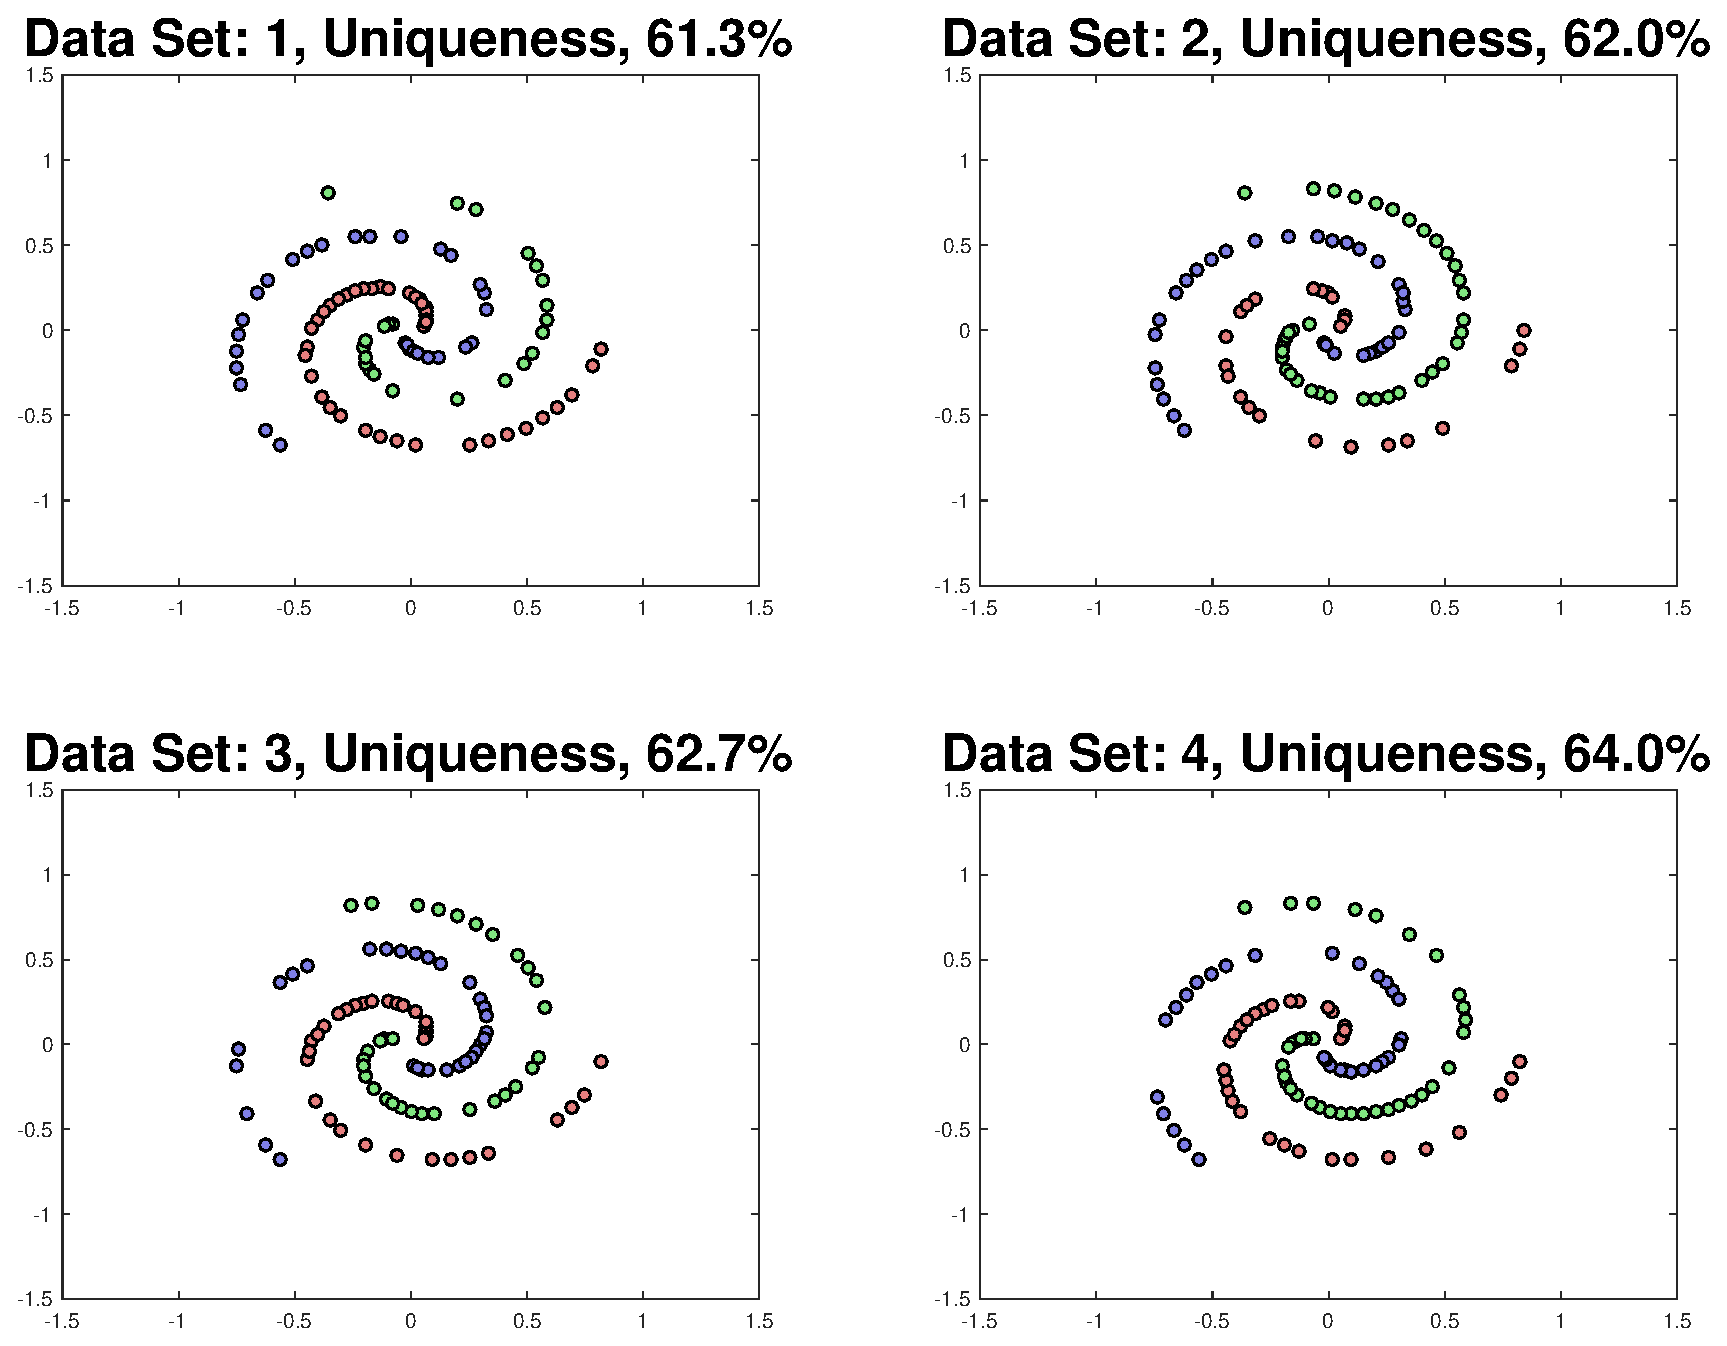
\includegraphics[width=0.60\columnwidth]{boot_strap}
    \caption{Overview of spectral subtraction process}
    \label{fig:boot_strap}
\end{figure}

The resulting data subsets sampled from the Toy Spiral data are shown in Figure \ref{fig:boot_strap}. Each dataset has 150 points however each spiral is not complete; some part of the spiral are miss, This is due to the fact that samples are drawn from the dataset with replacement. The amount of uniqueness in each dataset is captured in Figure \ref{fig:boot_strap} as well.  Ideally, as the size of our data set increases to $\infty$, the uniqueness percentage should approach $63.3\%$. The finite size of our dataset results in uniqueness values spread around the ideal. The table below shows the probability distributions of each class within the dataset. The roughly equal distributions corroborate the fact that sampling was done uniformly.

\begin{table}[H]
\centering
\begin{tabular}{|c|c|}
\hline
Dataset Index & Class Probabilitites 		\\ \hline
1             & $[0.3733, 0.2733, 0.3533]$  	\\ \hline
2             & $[0.2800, 0.3667, 0.3533]$  	\\ \hline
3             & $[0.3333, 0.3200, 0.3467]$ 	\\ \hline
4             & $[0.3467, 0.3133, 0.3400]$  	\\ \hline
\end{tabular}
\end{table}



The first step in the training of the decision forest is to develop the weak-learner functions that will be used to split the data at each node of the tree. Multiple weak-learner functions were implemented, namely axis-aligned and two-pixel. Linear, quadratic and cubic split functions were also implemented. Note that for the quadratic and cubic split functions have the form expressed in (\ref{eq:quad_split}) and (\ref{eq:cubic_split}) respectively.

\begin{align}
h(\textbf{v}, \theta) = [&a_1x_1^2+a_2x_2^2+a_3x_1x_2+a_4x_1+a_5x_2>\tau] \label{eq:quad_split} \\
h(\textbf{v}, \theta) = [&a_1x_1^3+a_2x_2^3+a_3x_1^2x_2+a_4x_1x_2^2+a_5x_1^2 \nonumber\\
&+a_6x_2^2+a_7x_1x_2+a_8x_1+a_9x_2>\tau] \label{eq:cubic_split}
\end{align}

The graphs below show the results obtained for all the weak-leaners tested, except for the two-pixel test. The two-pixel test works horribly when tested with this two dimensional data. Notice that the graphs obtained show the results when \texttt{param.splitNum} was set at 3. The results are indicative of the fact that a stronger class of learner functions does not necessarily translate into a greater information gain when the number of split functions tested is small.

\begin{figure}[H]
	\centering
    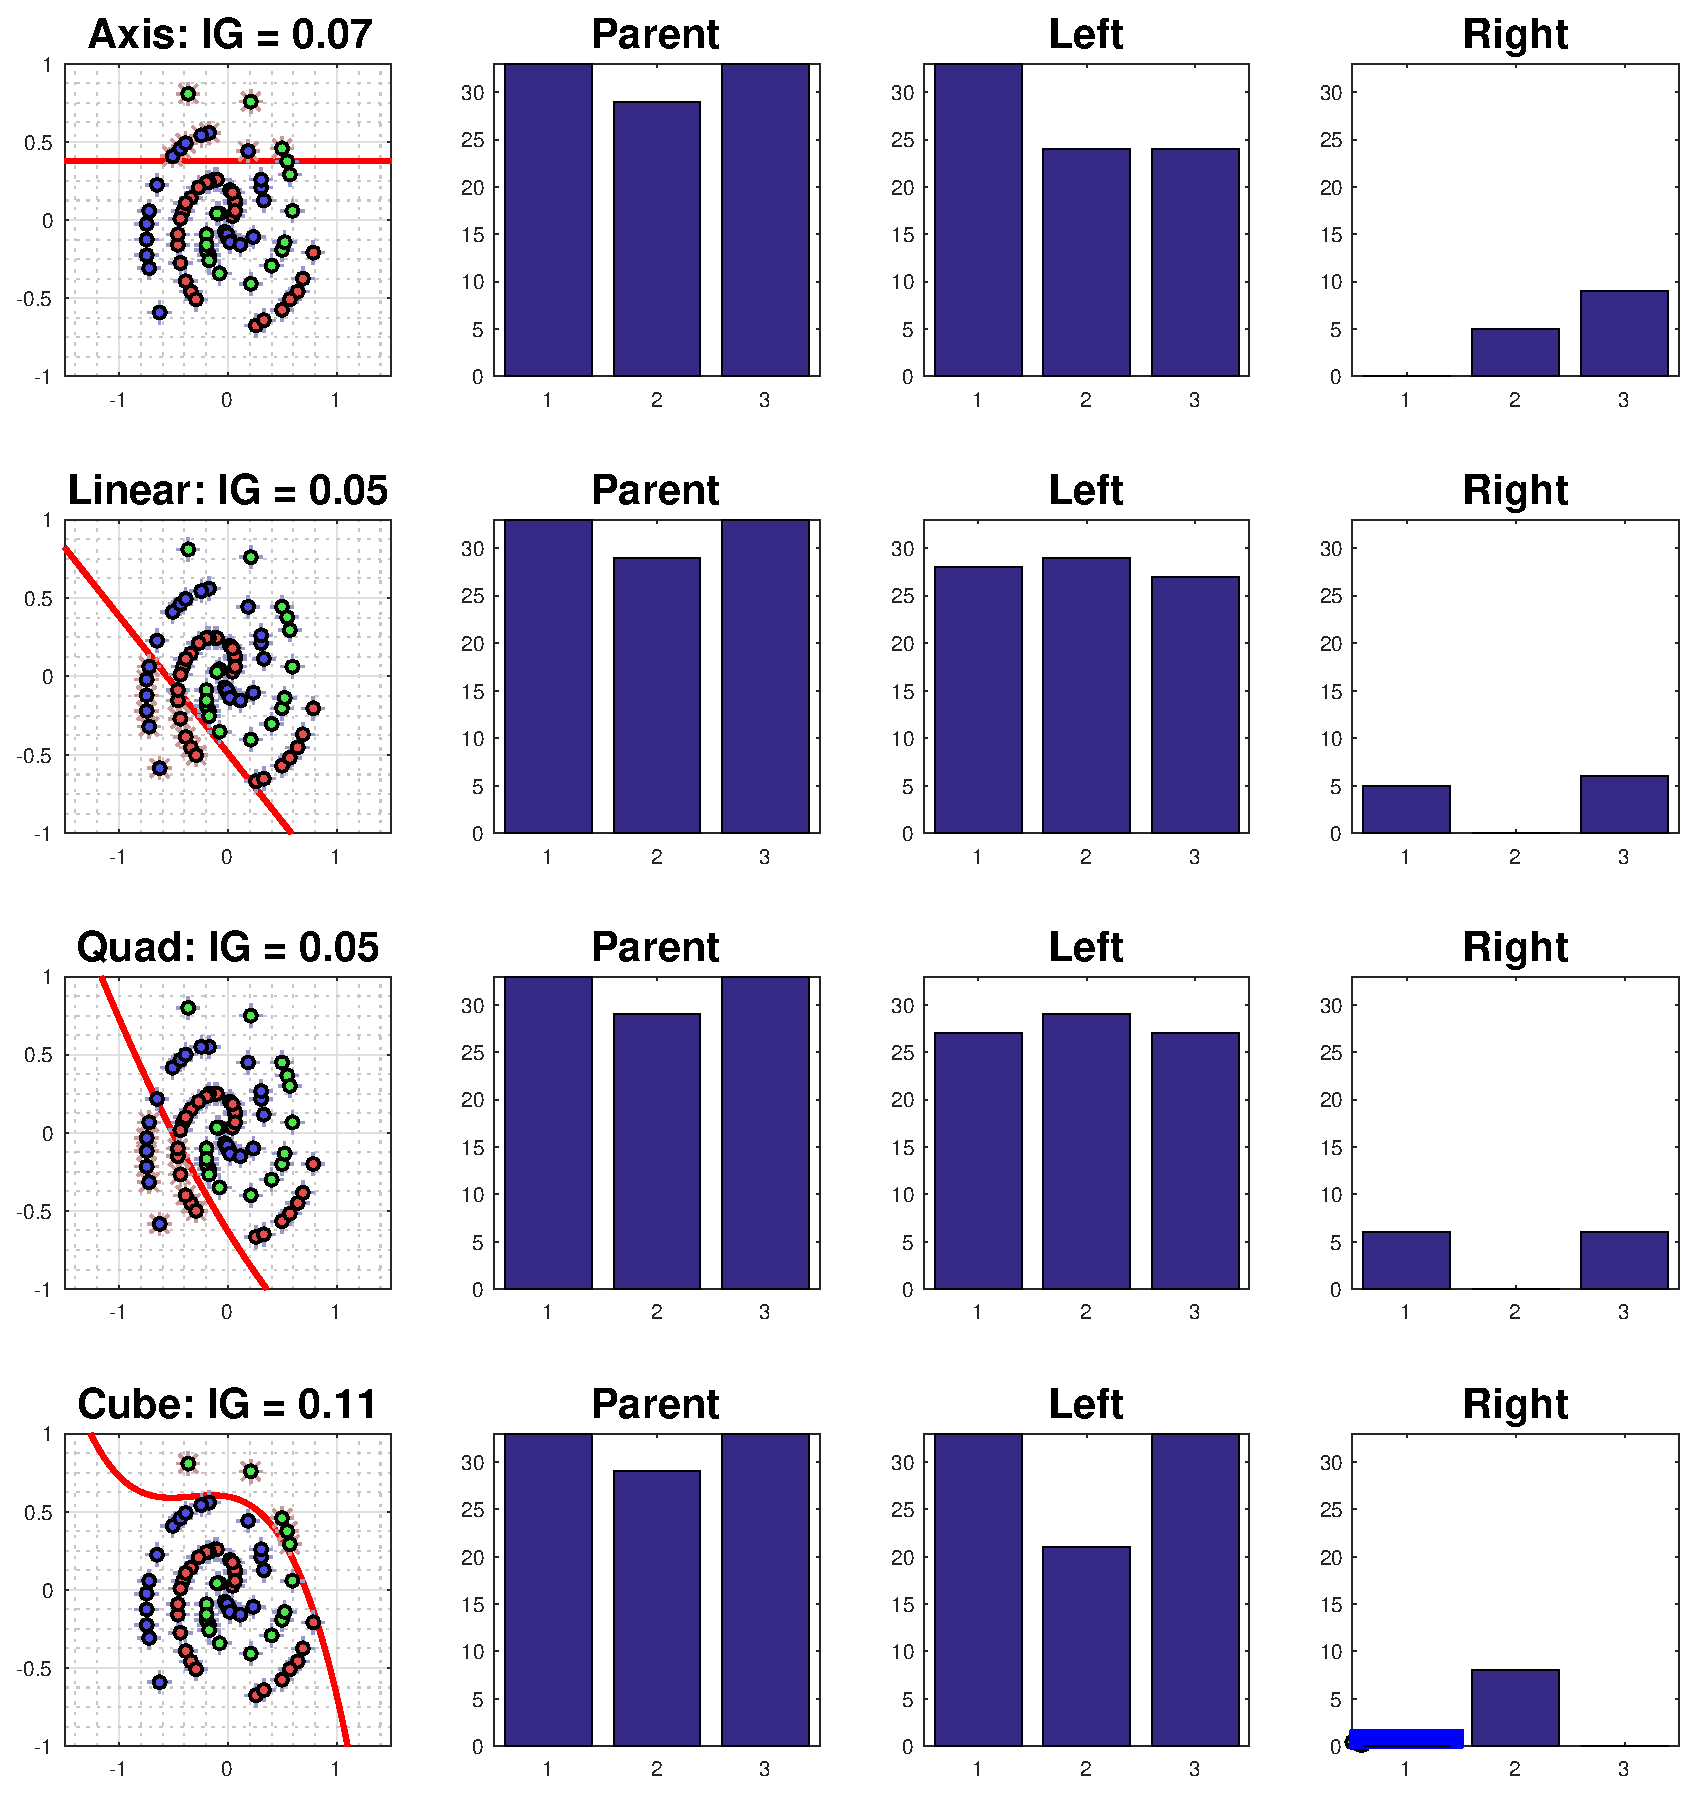
\includegraphics[width=0.60\columnwidth]{split_function_visualitions_1}
    \caption{Overview of spectral subtraction process}
    \label{fig:spec_sub_overview}
\end{figure}

The graph in Figure \ref{fig:spec_sub_overview} shows the effects that the strength of the learning class has when tested on nodes with a small number of data points. Observe the split function obtained for the quadratic learner. \textbf{There is clear over-fitting of the data.} In future sections, it should be noted that if stronger learning functions such as the quadratic non-linear learner are used, the number of trees should also be increased. An increase in the number of trees will allow the over-fitting that takes place to be averaged out. 

\begin{figure}[H]
	\centering
    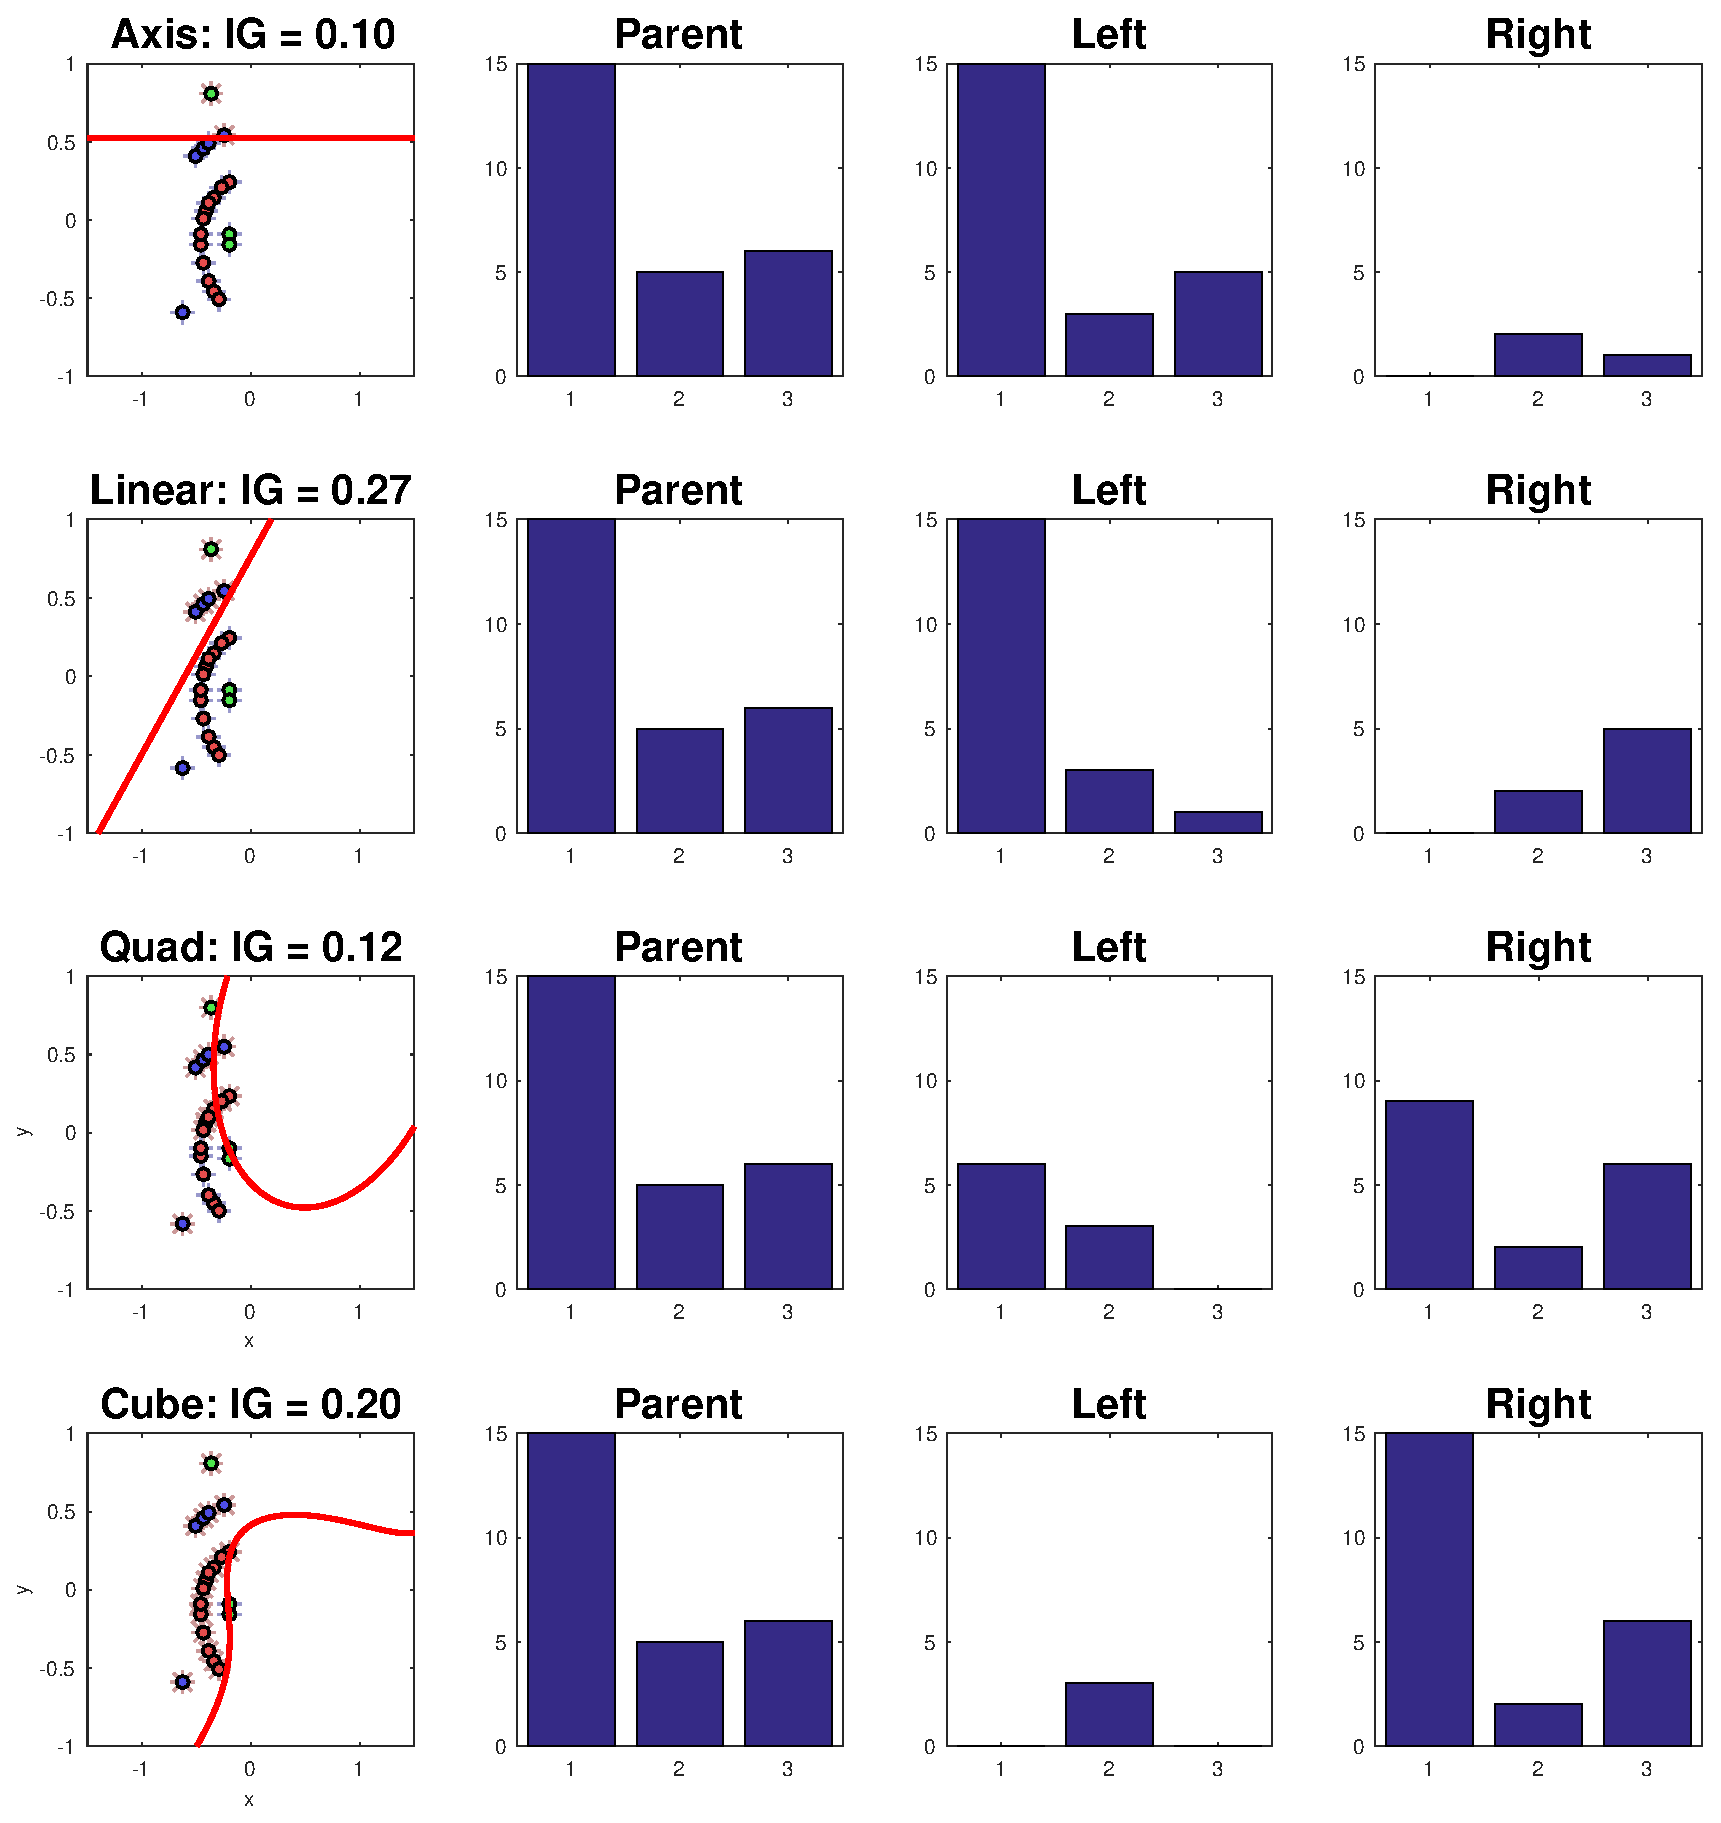
\includegraphics[width=0.60\columnwidth]{split_function_visualitions_3}
    \caption{Overview of spectral subtraction process}
    \label{fig:spec_sub_overview}
\end{figure}

Next, the \texttt{param.splitNum} is set to 20 and the results obtained are presented. It is clear a stronger learning class is able to split the data more efficiently and obtains a higher information gain. The discrimitative property of the learning classes is not obvious when the number of split functions tested is small however increasing \texttt{param.splitNum} clearly highlights the increased discriminative power. 

\begin{figure}[H]
	\centering
    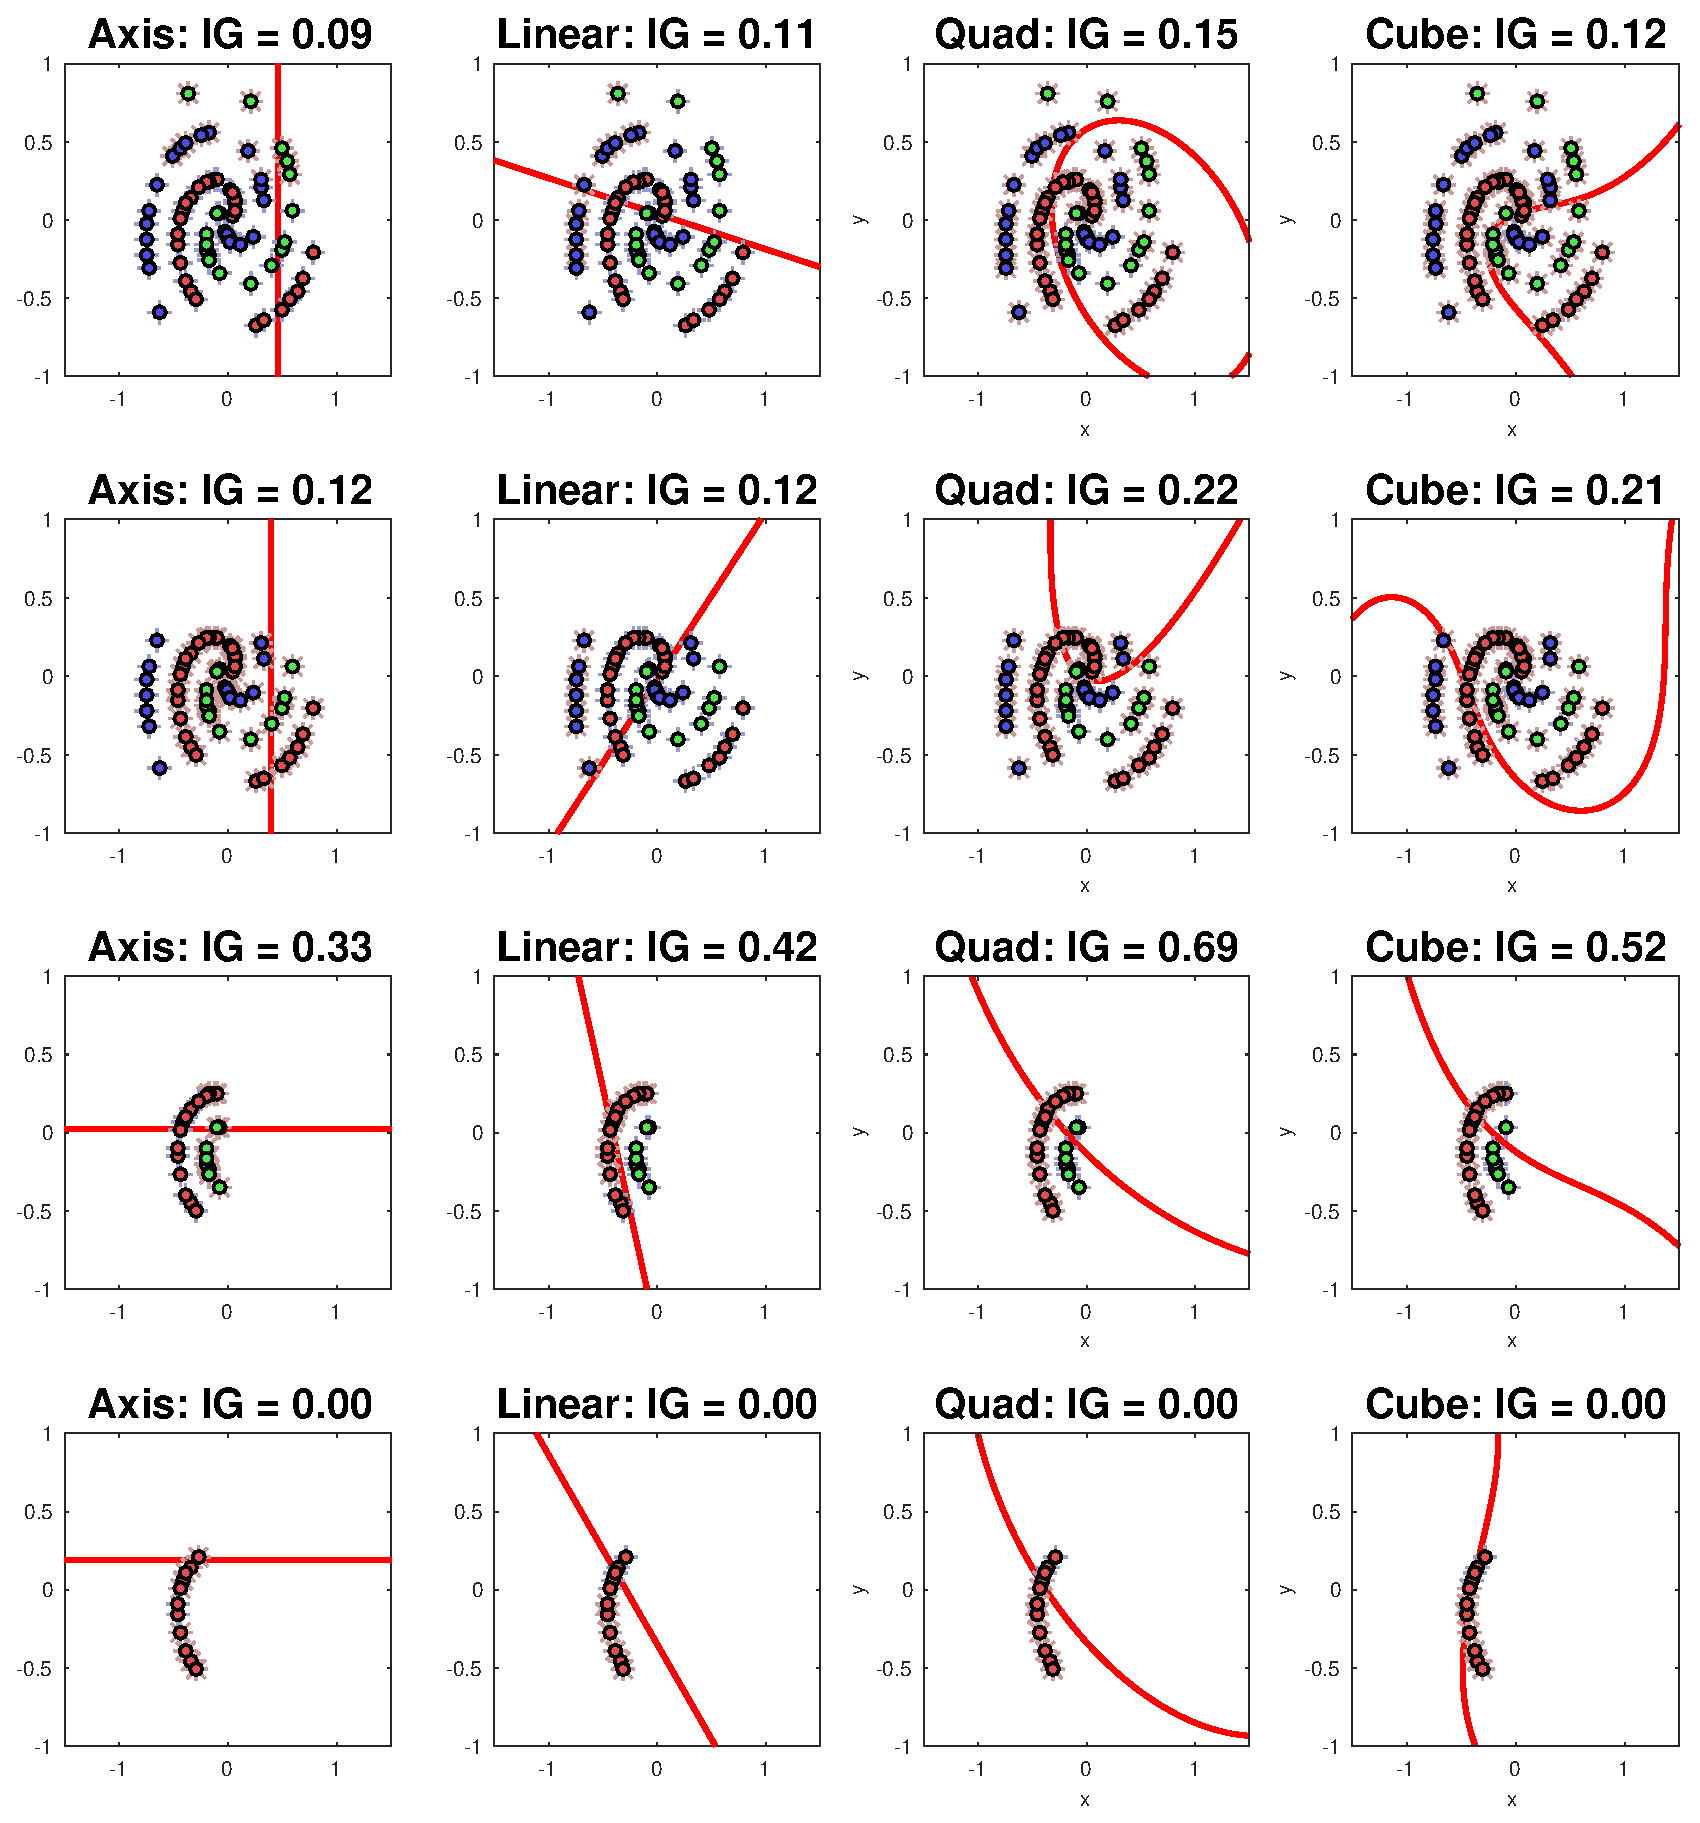
\includegraphics[width=0.60\columnwidth]{split_function_visualitions_5}
    \caption{Overview of spectral subtraction process}
    \label{fig:spec_sub_overview}
\end{figure}

Using a stronger learning class such as the quadratic or cubic non-linear functions has it benefits. They do lead to an increased information gain at each node. However, the increasing the strength of the learning class should also be accompanied with a small increase in the number of split functions tested. Stronger class have more degrees of freedom and thus search for a linear seperator in a higher dimensional space. As such, keeping the number of split functions that we test constant is not ideal.


Lastly, the leaf nodes have been visualized in Figure \ref{fig:leaf_nodes}. The leaf nodes have been generated using the axis-aligned weak learner with \texttt{param.splitNum} set to 3. It is clear that the leaf nodes mostly contain only one class of data points; the recursive splitting of the data points down the tree has a distilling effect. There are still leaf nodes with 2 or more classes of data, these nodes could be attributed to the region near the middle of the Toy Spiral where the data points are more tightly clustered.

\begin{figure}[H]
	\centering
    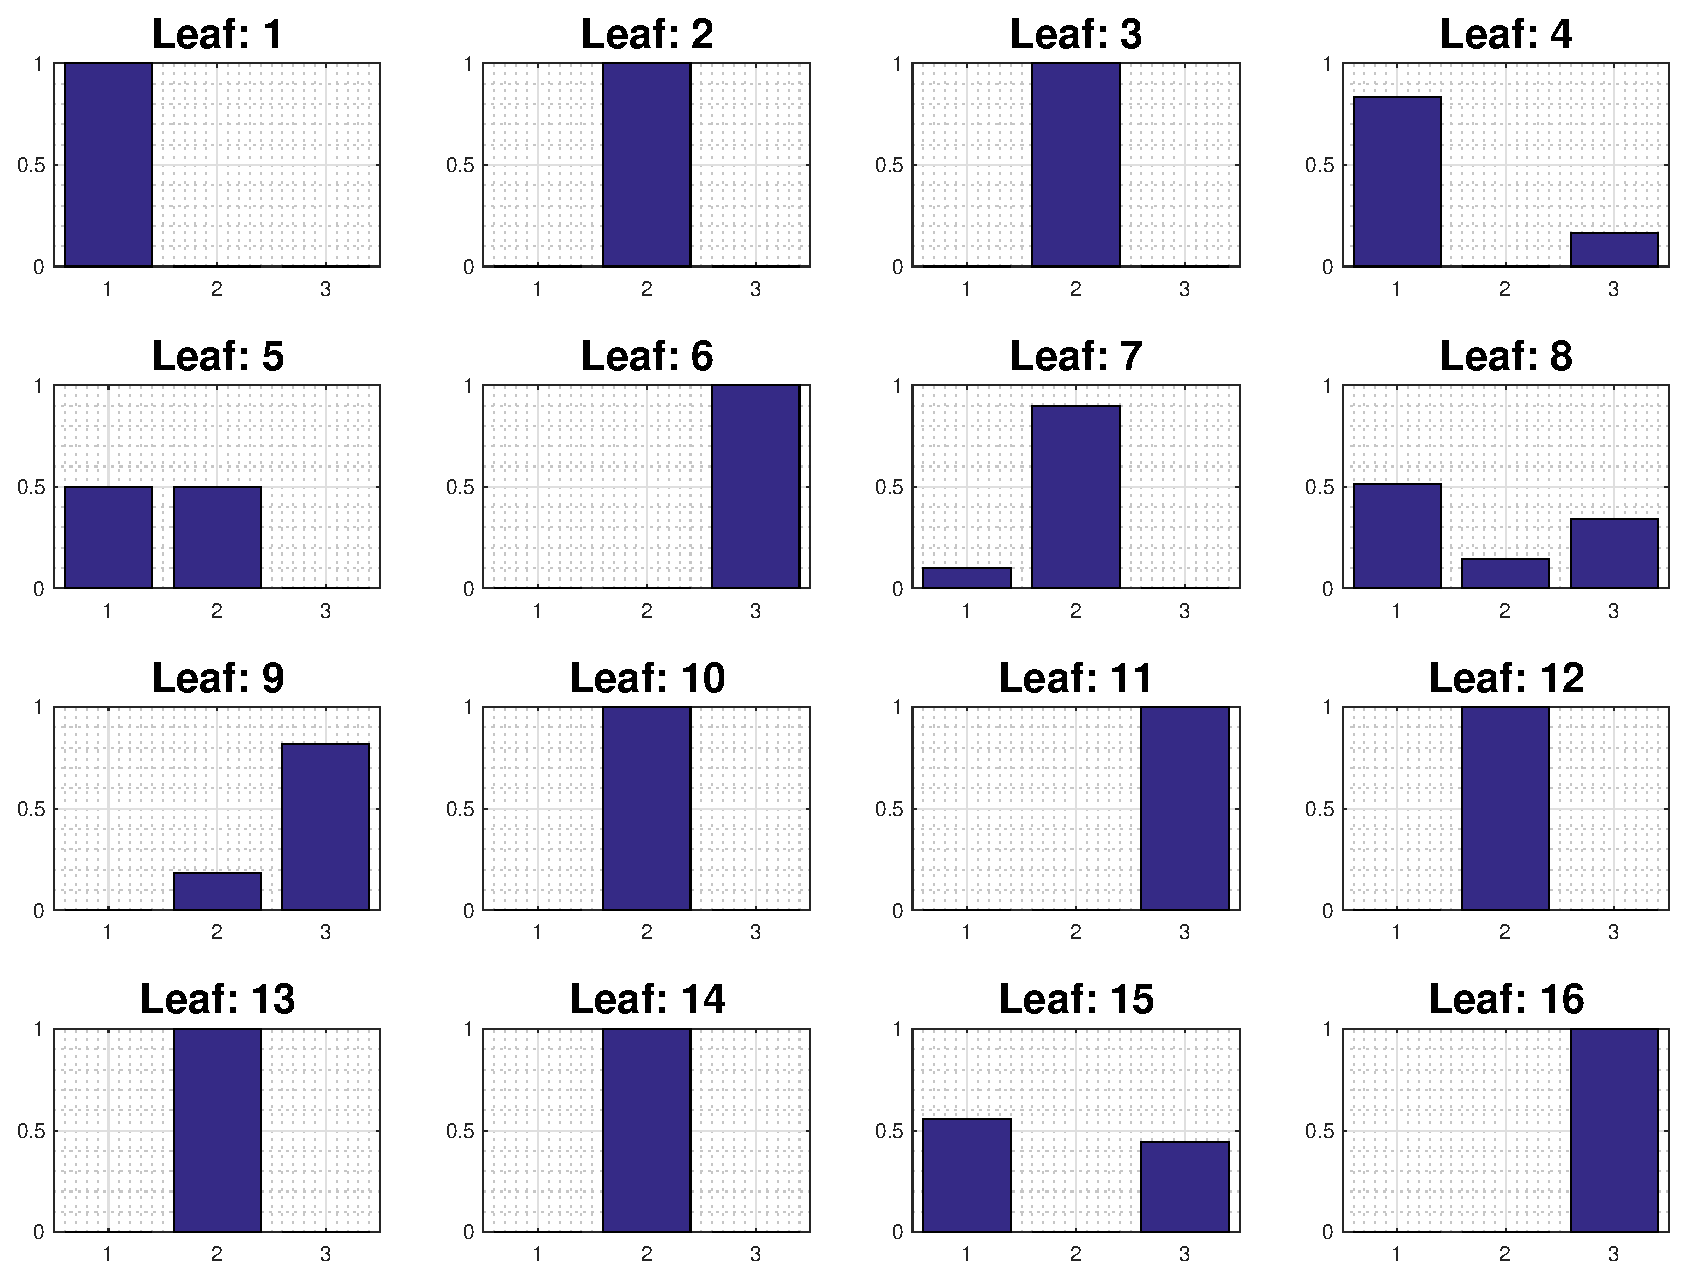
\includegraphics[width=0.60\columnwidth]{leaf_node_distributions_1}
    \caption{Overview of spectral subtraction process}
    \label{fig:leaf_nodes}
\end{figure}

\section{Evaluating Decision Forest}

The first parameter that is varied is the number of trees in the forest. The graph below shows that increasing the number of trees has a considerable effect on the classification process for when the absolute number of trees is small. Increasing the number of tress from 100 to 200 has negligible effect. Notice the straight class boundaries obtained in the region of the grid for which extrapolation is required. All training data is contained within the unit square whereas the region for which the classifier is tested extends beyond the unit sqaure. For that reason, the classifier is expected to extrapolate the class boundaries. Since the axis-aligned weak learner is used, the extrapolation leads to straight axis-aligned lines. 

\begin{figure}[H]
	\centering
    \includegraphics[width=0.40\columnwidth]{ax_5_trees}
	\includegraphics[width=0.40\columnwidth]{ax_20_trees}
    \includegraphics[width=0.40\columnwidth]{ax_100_trees}
    \includegraphics[width=0.40\columnwidth]{ax_200_trees}
    \caption{Overview of spectral subtraction process}
\end{figure}

Next, we vary the number of split functions, keeping the number of trees fixed at $10$. Notice that by increasing the number of split functions tried, we are decreasing the randomness of inherent in each tree. The ensemble learner's variance depends on tree being highly uncorrelated. Increasing the number of split functions to $9$, the random forest has highly over-fit the green class. Notice how much lower the class boundary between the red and green class now is.

\begin{figure}[H]
	\centering
    \includegraphics[width=0.40\columnwidth]{splitNum_3}
	\includegraphics[width=0.40\columnwidth]{splitNum_5}
    \includegraphics[width=0.40\columnwidth]{splitNum_7}
    \includegraphics[width=0.40\columnwidth]{splitNum_9}
    \caption{Overview of spectral subtraction process}
\end{figure}

The third parameter in that can be varied is the depth of the tree. It can be seen that more accurate results are produced when tree depth is increased. With tree depth set at 3 or 5, there are very obvious artifacts that appear; a thin red line when depth is set at 3, and a massive blue region when the depth is set at 5. These are clearly anomalies that have come about because the classes have not been sufficiently refined at the leaf nodes. Increasing the depth to 7, the obvious anomalies have now disappeared by small artifacts still remain at the center of the graph. These can be further refined if the tree depth is increased to 9. With tree depth at 9, it is abantantly clear that the random forest is not mimicing the non-linear spiral behavior using the axis-aligned weak learner. 

\begin{figure}[H]
	\centering
    \includegraphics[width=0.40\columnwidth]{tree_depth_3}
	\includegraphics[width=0.40\columnwidth]{tree_depth_5}
    \includegraphics[width=0.40\columnwidth]{tree_depth_7}
    \includegraphics[width=0.40\columnwidth]{tree_depth_9}
    \caption{Overview of spectral subtraction process}
\end{figure}

Note that all the discussion above has all been made with respect to the axis-aligned weak learner. This is important to note that ideal values of splitNum and the tree depth vary with the weak learner used. Note the graph below, which uses the 


\end{document}